\section{Δυαδικά προγράμματα επεξεργασίας κειμένων}
Τα δυαδικά προγράμματα επεξεργασίας κειμένων ή αλλιώς hex editors αποτελούν εφαρμογές για την τροποποίηση και την κατανόηση προγραμμάτων τα οποία έχουν μεταφραστεί σε γλώσσα μηχανής.
H ονομασία "hex" (hexadecimal) ή δεκαεξαδίκο είναι σύστημα αρίθμησης με βάση το δεκαέξι.
Περιέχει τους βασικούς αριθμούς 0-9 και τα γράμματα A-F.
Το συγκεκριμένο σύστημα αρίθμησης χρησιμοποιείται ευρέως καθώς αντιπροσωπεύει σε πολύ καλό βαθμό τις δυαδικά κωδικοποιημένες τιμές \emph{(binary-coded values)}.
Υπάρχουν ποικίλες υλοποιήσεις των συγκεκριμένων προγραμμάτων με έμφαση σε διαφορετικά σενάρια.

Το παρόν κεφάλαιο θα μελετήσει τις λειτουργίες και τα χαρακτηριστικά των διορθωτών που υπάρχουν στο διαδίκτυο σαν \emph{freeware} ή  \emph{free and open source}.
Επίσης θα θέσει μια κατευθυντήρια γραμμή με βάση τις απαιτήσεις και τις λειτουργίες στην οποία θα βασιστεί ο καινούργιος διορθωτής hex.

\pagebreak
\subsection{HxD Editor}
Το \emph{HxD Hex Editor}\cite{hxd} είναι ένας επεξεργαστής που διανέμεται ελεύθερα \emph{(freeware)} και έχει σχεδιαστεί για την πλατφόρμα των \emph{Windows}.
Από την γραφική διεπαφή μπορεί να αλλάξει κάποιος κωδικοποίηση μεταξύ πολλών κωδικοποιήσεων 8-bit.
Από τις βασικές λειτουργίες, ο επεξεργαστής υποστηρίζει τις κλασσικές λειτουργίες ίδιου είδους προγραμμάτων όπως: αντιγραφή, επικόλληση, εύρεση και αντικατάσταση ή μετάβαση στη διεύθυνση.
Μπορεί επίσης να διαχειριστεί μεγάλα σε μέγεθος αρχεία ή επεξεργασία τμημάτων μνήμης ή και δίσκου, συνένωση ή διαχωρισμό αρχείων \emph{splitting - concat} όπως επίσης και στατιστικών μετρήσεων.

Ωστόσο, ο συγκεκριμένος διορθωτής υποστηρίζει σαν λειτουργικό σύστημα μόνο \emph{Windows}.
% Ενδέχεται να χρειάζεται βιβλιογραφική αναφορά
Βέβαια σε περιβάλλον \emph{linux} ή {macOS} ενδείκνυται η αξιοποίηση βιβλιοθηκών τα οποία λειτουργούν σαν επίπεδα συμβατότητας \emph{compatibility layer} όπως το wine \emph{(Wine Is Not an Emulator)} και το \emph{crossover} ή το {bootcamp} αντίστοιχα.

Τέλος ο συγκεκριμένος editor διαθέτει πολλές μεταφράσεις σε ξένες γλώσσες και μια από αυτές είναι η ελληνική η οποία δεν είναι ολοκληρωμένη.

\begin{figure}[ht]
\centering
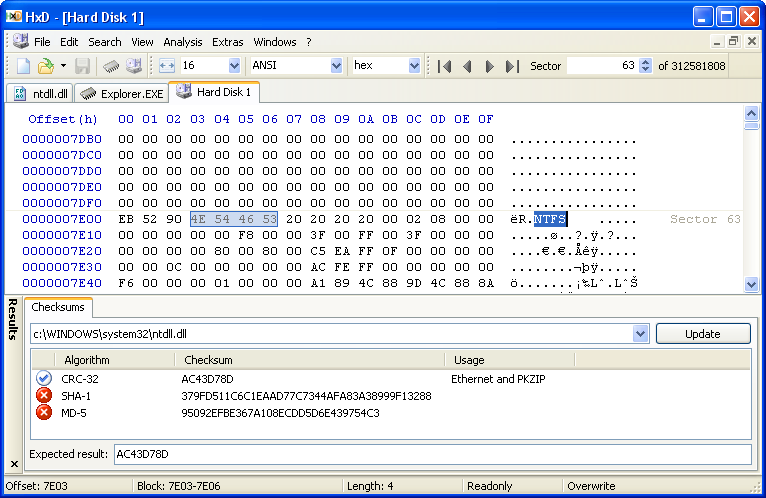
\includegraphics[scale=0.5]{static/hxd.png}
\caption{HxD - Freeware Hex Editor and Disk Editor}
\end{figure}

\pagebreak
\subsection{Hexed.it}
Το \emph{hexed.it}\cite{hexedit} είναι ένας free hex editor ο οποίος λειτουργεί σαν web app στον περιηγητή ιστού.
Αυτός ο \emph{editor} προσφέρει λειτουργία χωρίς σύνδεση στο διαδίκτυο καθώς όλο το εκτελέσιμο τρέχει από την μεριά του χρήστη \emph{(client side execution)}.

Επιτελεί και αυτός τις βασικές λειτουργίες ενός hex editor όπως εισαγωγή, αντικατάσταση, ανάζητηση συγκεκριμένης διεύθυνσης \emph{(goto)}, απεριόριστα \emph{undo-redo} οριοθετημένα από τις δυνατότητες του εκάστοτε περιηγητή.
Ακόμα είναι ικανό να ανοίγει μεγάλα αρχεία της τάξης των \emph{gigabyte} ακόμα και αν δεν υπάρχει διαθέσιμη μνήμη ram και να αναγνωρίζει την πλειοψηφία από τους τύπους αρχείων που κυκλοφορούν.
Επίσης έχει την δυνατότητα της επιθεώρηση (data inspection) σε κάθε μεμονωμένο byte και ο χρήστης να βλέπει την τιμή του σε 8,16,32,64-bit αναπαράσταση.

\begin{figure}[ht]
\centering
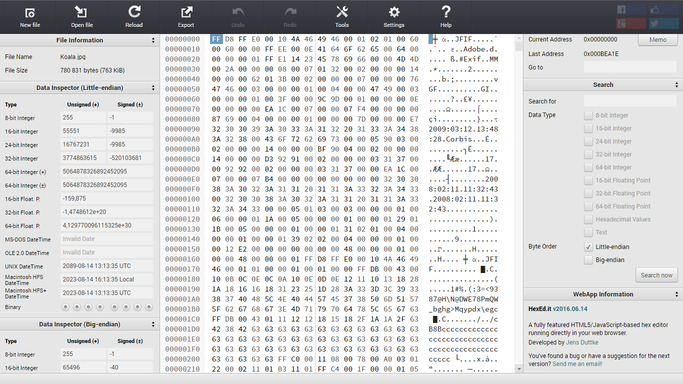
\includegraphics[scale=0.5]{static/hexedit.png}

\caption{HexEd.it: A full featured HTML5/javascript-based hex editor running directly from your browser}
\end{figure}

\pagebreak
\subsection{wxHexEditor}
Το wxHexEditor\cite{wxhex} είναι ένα πρόγραμμα επεξεργασίας (hex editor) ανοιχτού κώδικα με μεγάλη υποστήριξη αρχείων. 
Η γραφική διεπαφή επιτρέπει στον χρήστη να επιλέξει μεταξύ διαφορετικών κωδικοποιήσεων, από ASCII έως UTF παραλλαγές.
Ωστόσο, η επεξεργασία κειμένου είναι δυνατή μόνο σε κωδικοποίηση ASCII.
Ο συντάκτης περιλαμβάνει έναν μεταγλωττιστή δεδομένων με υποστήριξη για βασικούς τύπους δεδομένων και εναλλαγή endianity.
Εκτός από αυτές τις λειτουργίες, προσφέρει επίσης τη δυνατότητα σήμανσης τμημάτων δεδομένων χρησιμοποιώντας ετικέτες,ανάγνωση δεδομένων ως οδηγίες συναρμολόγησης (assembly), ανάγνωση δεδομένων από μνήμη (ram) συγκεκριμένης διαδικασίας.

Ένα άλλο πλεονέκτημα αυτού του προγράμματος επεξεργασίας είναι η διαθεσιμότητα μεταφράσεων σε ξένες γλώσσες.
Το wxHexEditor υποστηρίζει πλατφόρμες \emph{MS Windows, Mac OS και Linux}.
Παρά τον μεγάλο αριθμό λειτουργιών , ο editor βρίσκεται ακόμη σε έκδοση beta και μπορεί να χρησιμοποιηθεί απλώς αντιμετωπίζει προβλήματα σταθερότητας.

\begin{figure}[ht]
\centering
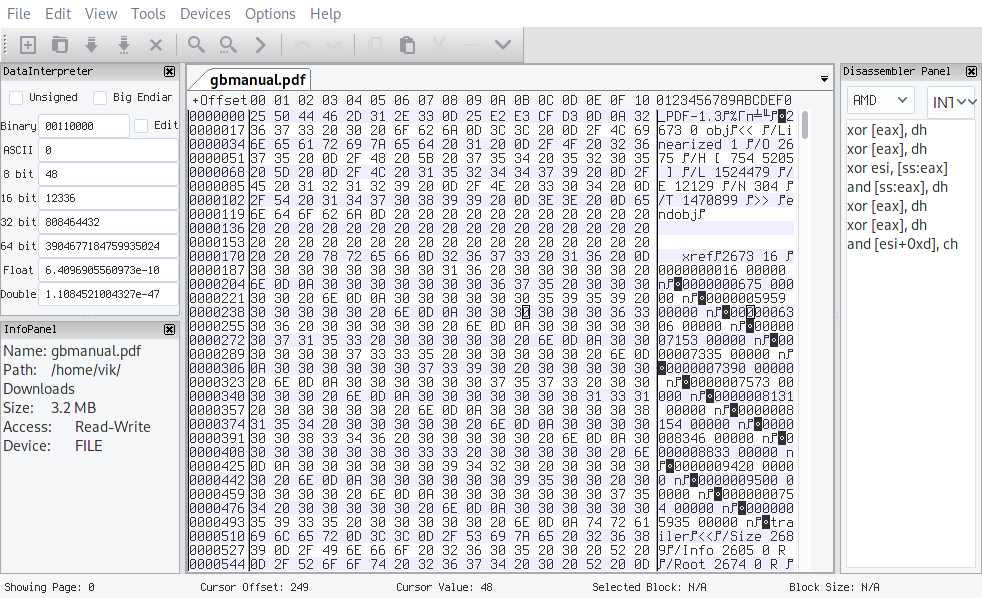
\includegraphics[scale=0.5]{static/wxhex.png}

\caption{wxHedEditor}
\end{figure}

\pagebreak
\subsection{rehex: Reverse Engineer's hex editor}
Το \emph{rehex} \cite{rehex} είναι ένας σύγχρονος hex editor ανοιχτού και ελεύθερου λογισμικού.
H αρχική σελίδα του λογισμικού δίνει την περιγραφή ως \emph{Ένας hex editor πολλαπλών πλατφορμών (Windows, Linux, Mac) για reverse engineering και οτιδήποτε άλλο}.

Ο συγκεκριμένος editor διαθέτει αρκετά παρόμοιες λειτουργίες με την λίστα των editor που έχουμε περιγράψει έως τώρα.
Σημαντικό χαρακτηριστικό που τον αναδεικνύει από τους προηγούμενους είναι η δυνατότητα που έχει ο χρήστης για \emph{inline dissasembly} της γλώσσας μηχανής.
Διαθέτει και αυτός υποστήριξη για μεγάλα αρχεία της τάξης του 1TB+ όπως επίσης και την δυνατότητα scripting με κάποια εξωτερίκη γλώσσα προγραμματισμού.

\begin{figure}[ht]
\centering
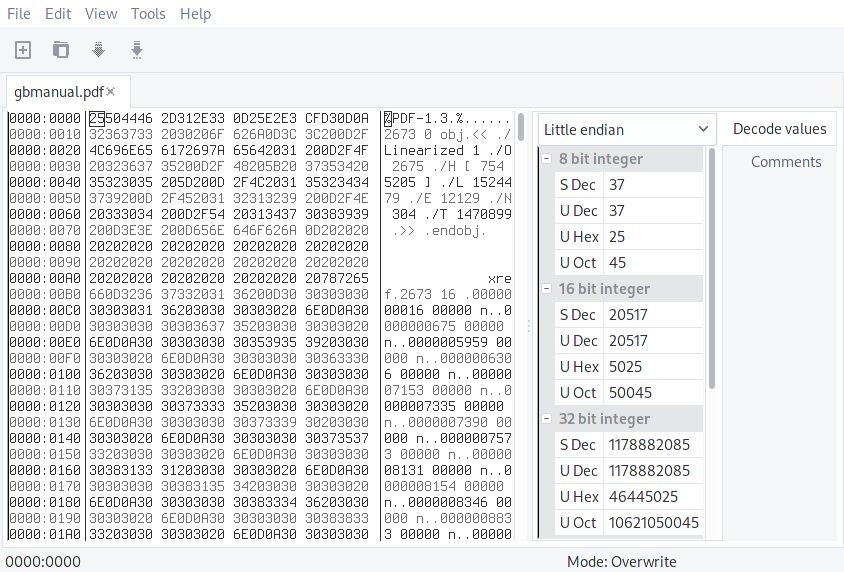
\includegraphics[scale=0.5]{static/rehex.png}

\caption{rehex: Reverse Engineer's hex editor}
\end{figure}

\pagebreak
\subsection{Περίληψη λειτουργιών}
Ο παρακάτω πίνακας συγκρίνει τις επιλεγμένες λειτουργίες επεξεργαστή.
Κάθε λειτουργία θα σημειώνεται για κάθε hex editor που την υλοποιεί

\begin{table}[h!]
\centering
\begin{tabular}{|c|c c  c  c|} 
    \hline
    Λειτουργίες & HxD & HexEd.it & wxHexEditor & Rehex \\ [0.5ex] 
    \hline
    Αντιγραφή και επικόλληση    & \times & \times & \times & \times \\ 
    Βρίσκω και αντικαθιστώ      & \times & \times & \times & \times \\
    Κάνε πίσω                   & \times & \times & \times & \times \\
    Υποστήριξη μεγάλων αρχείων  & \times & \times & \times & \times \\
    Μεταγλωττιστής δεδομένων    & - & \times & \times & \times \\
    Αναγνώριση μορφής           & - & - & \times & \times \\
    Go to                       & \times & \times & \times & \times \\
    Inline disassembly          & \times & \times & \times & \times \\
    
    \hline
\end{tabular}
\caption{Λειτουργίες hex editor}
\end{table}

Συμπερασματικά, με βάση τους στόχους και τις λειτουργίες που είχαμε ορίσει στις απαιτήσεις του προγράμματος διαπιστώνουμε ότι από τους τέσσερις μόνο οι δυο hex editor υποστηρίζουν την λειτουργικότητα αναγνώρισης μορφής αρχείου.

Η προγραμματιστική υλοποίηση της πτυχιακής βασίστηκε και έγινε με την βοήθεια ενός text editor του kilo\cite{kilo}.
H συγκεκριμένη επιλογή έγινε αφενός από την αρκετά ολοκληρωμένη τεκμηρίωση του κώδικα (\emph{documentation}) αφετέρου από την επιλογή της γλώσσας προγραμματισμού την \textbf{C} που επιλέχθηκε για να γραφτεί ο \emph{text editor}.
Επίσης ο συγκεκρίμενος \emph{text editor} στοχεύει το τερματικό το οποίο αποτελεί μια πρoϋπόθεση για τον \emph{hex editor} της πτυχιακής.
Περιέχει αρκετά χρήσιμες \emph{non-trivial} συναρτήσεις που αφορούν την εύκολη αλληλεπίδραση με το περιβαλλόν του τερματικού τις οποίες δανείστηκε η υλοποίηση μου.

Υπάρχει και μια άλλη λειτουργικότητα προς υλοποίηση, η ανίχνευση επαναχρησιμοποίησης κώδικα \textbf{binary code reuse detection}. Για την επαναχρησιμοποίηση κώδικα πρέπει να στραφεί η προσοχή σε αλγόριθμους με τα χαρακτηριστίκα \textbf{binary diffing}. Συγκεκριμένα, επιλέχθηκαν τρεις επιστημονικές αναφορές που θα περιγραφούν παρακάτω. 

\pagebreak
\subsection{Ανίχνευση επαναχρησιμοποιήσης κώδικα}
Ο ορισμός του software reverse engineering αποδίδεται σύμφωνα με το Ινστιτούτο Ηλεκτρολόγων και Ηλεκτρονικών Μηχανικών \emph{IEEE} ως 
\say{η διαδικασία ανάλυσης ενός υποκείμενου συστήματος για τον προσδιορισμό των συστατικών του συστήματος και των συσχετισμών τους και για τη δημιουργία αναπαραστάσεων του συστήματος σε άλλη μορφή ή σε υψηλότερο επίπεδο αφαίρεσης"}\cite{reverse}
στο οποίο το "υποκείμενο σύστημα" αποτελεί το τελικό προϊόν της ανάπτυξης κώδικα \emph{software development}.

% Should put a figure 

Στο συγκεκριμένο κεφάλαιο θα γίνει μια επισκόπηση τριών επιστημονικών άρθρων της τεχνικής \emph{binary code reuse detection}.
% Μια σύντομη περιγραφή των paper ακολουθεί παρακατω.
Κάθε μία από τις υλοποιήσεις που προτείνονται στα κείμενα βασίζονται σε διαφορετικές δομές δεδομένων.
Για παράδειγμα, στην υλοποίηση του bitshred\cite{bitshred} χρησιμοποιείται ένα \emph{bloom filter} το οποίο είναι μία δομή που απαρτίζεται από συναρτήσεις κατακερματισμού και πίνακες bit. Από την άλλη το binsequence χρησιμοποιεί κατευθυνόμενους γράφους.

\pagebreak
\subsection{BitShred}
To paper `\emph{BitShred: feature hashing malware for scalable triage and semantic analysis}`\cite{bitshred} προτείνει έναν ελαφρύ και scalable αλγόριθμο ανίχνευσης επαναχρησιμοποίησης κώδικα. Συνοπτικά τα βήματα που ακολουθεί για να επιτελέσει το έργο του είναι:

\begin{enumerate}
    \item Θρυμματίζει το αρχείο \emph(shredding).
    \item δημιουργεί αποτυπώματα (\emph{fingerprints}). 
    \item συγκρίνει τα αποτυπώματα.
\end{enumerate}

Σε αρχικό στάδιο, τεμαχίζει (\emph{shredding}) το αρχείο, αναλύοντας και εντοπίζοντας το εκτελέσιμο κομμάτι του binary.
Έπειτα διαχωρίζει τα κομμάτια σε θραύσματα (\emph{shreds}) τα οποία αποτελούν συνεχόμενες ουρές byte μήκους n, που συνήθως αποκαλούνται (\emph{n-gram}).

% Bloom filter
Για να είναι αποδοτικός ο αλγόριθμος μέχρι και σε ογκώδη προγράμματα, η αποθήκευση των θραυσμάτων γίνεται με την χρήση των \emph{bloom filters}.
Ας υποθέσουμε ότι υπάρχει ένα σύνολο δεδομένων S.
Ένα bloom filter μπορεί να κρίνει εάν ένα στοιχείο \textbf{x} είναι μέλος του \textbf{S} με αποδοτικό τρόπο αποθήκευσης.
Τα bloom filters δεν έχουν ψευδή αρνητικά (\emph{false negatives}) δηλαδή, οι δοκιμές συμμετοχής δεν επιστρέφουν ποτέ x \nexists \space \textbf{S} όταν \textbf{x} είναι πραγματικά μέλος του \textbf{S}.
Στον πυρήνα τους αποτελούνται από \emph{μ} πίνακες \emph{bit} και \emph{ν} διαφορετικές συναρτήσεις κατακερματισμού.
Αρχικά, όλα τα bit του θέτονται 0.
Η πρόσθεση ενός στοιχείου απαιτεί την εφαρμογή \textbf{k} hash functions στο στοιχείο και τα bit τα οποία ευ}ρετηριάζονται από τις προκύπτουσες τιμές κατακερματισμού ορίζονται σε 1.
Αφού προσθέσουμε όλα τα shreds στον bloom filter ο ίδιος θεωρείται πλέον το αποτύπωμα (fingerprint) του αρχείου.

% Main algorithm
Στο τελευταίο στάδιο, για να υπολογίσουμε την ομοιότητα μεταξύ των αρχείων χρησιμοποιείται ο δείκτης \textbf{Jaccard}.
O δείκτης ορίζεται ως το μέγεθος τομής δύο δειγμάτων δια το μέγεθος ένωσης δύο δειγμάτων:

{\centering
{\normalsize $J(A, B) = \displaystyle \frac{|A\space\cap B|}{|A\space\cup B|}$} \par
} Με άλλα λόγια, εάν έχει οριστεί ένα συγκεκριμένο bit του \emph{A}, τότε το αντίστοιχο χαρακτηριστικό του \emph{A} είναι 1 αλλιώς είναι 0. Έτσι, ο δείκτης Jaccard μπορεί να υπολογιστεί ως εξής:


{\centering
{\normalsize $J(A, B) = \displaystyle \frac{F_{11}}{F_{01} + F_{10} + F_{11}}$} \par
}

όπου $F_{11}$: ο συνολικός αριθμός bit που ορίζονται τόσο από το \emph{A} όσο και από το \emph{B}, $F_{01}$: ο συνολικός αριθμός bit μόνο από το \emph{B} , $F_{10}$: ο συνολικός αριθμός bit μόνο από το \emph{A}.


\pagebreak
\subsection{BinJuice}
Σε αυτό το κεφάλαιο θα μελετήσουμε την επιστημονική αναφορά \emph{`Fast location of similar code fragments using semantic 'juice'}`\cite{binjuice}.
Με τον όρο \emph{juice} το συγκεκριμένο paper εννοεί μια γενίκευση της σημασιολογίας (\emph{semantics}) ενός προγράμματος.
Ο `χυμός` λαμβάνει υπόψη τις βασικές σχέσεις που δημιουργούνται από ένα κομμάτι κώδικα, ανεξάρτητα από τις επιλογές των καταχωρητών και των σταθερών.
Ο `χυμός` στη συνέχεια χρησιμεύει ως πρότυπο του κώδικα που είναι αμετάβλητο έναντι συγκεκριμένων επιλογών από τους μεταγλωττιστές (\emph{compilers}) ή με εργαλεία κωδικοποίησης κώδικα (\emph{code obfuscation tools}).

Η διαδικασία εξαγωγής \emph{binary juice} από ένα εκτελέσιμο αρχείο αποτελείται από τα ακόλουθα βήματα:
\begin{itemize}
	\item Αποσυναρμολόγηση \emph{(disassembly)} του binary.
	\item Αποσύνθεση του αποσυναρμολογημένου προγράμματος σε διαδικασίες (\emph{procedures}) και block.
	\item Υπολογισμός της σημασιολογίας ενός block.
	\item Υπολογισμός του \emph{juice} ενός block.
\end{itemize}

Για το πρώτο βήμα, έτσι όπως περιγράφεται στην αναφορά χρησιμοποιούνται εργαλεία όπως το IDA PRO\cite{ida} και το objdump\cite{objdump}.
To disassembly που παράγεται από το τα προαναφερθέντα εργαλεία \emph{(και άλλα)} δεν εγγυώνται oλοκληρωμένες λύσεις.
Ως εκ τούτου το ποσοστό πληρότητας της σημασιολογίας και των υπολογισμών του χυμού βασίζονται σε ακριβείς λύσεις από τα δύο πρώτα βήματα.

Το αποτέλεσμα της αποσύνθεσης του δεύτερου βήματος πρέπει να αντιπροσωπεύει ένα γράφημα ροής ελέγχου (\emph{Control Flow Graph}).
Ένας κόμβος αυτού του γραφήματος είναι ένα μπλοκ: μια ακολουθία από instructions έτσι ώστε εάν η εκτέλεση ξεκινά από τo πρώτo , ο έλεγχος θα περάσει μέχρι και το τελευταίο instruction και θα τερματίσει.
Η σημασιολογία (\emph{ή χυμός}) μιας διαδικασίας αποτελείται από ένα ισομορφικό γράφημα των οποίων οι κόμβοι αντιπροσωπεύουν τη σημασιολογία (ή χυμό) του αντίστοιχου κόμβου στο CFG.
Όπως είναι εύλογο, η ουσία του αλγορίθμου έγκειται στον υπολογισμό της σημασιολογίας-χυμού των μεμονωμένων block.

Το τρίτο βήμα, αφορά τον υπολογισμό του χυμού των μπλοκ και των διαδικασιών με την χρήση ενός συμβολικού διερμηνέα (\emph{symbolic interpreter}) με τον όρισμο:

{\centering
	Interpret:seq(Instruction) x State \rightarrow\space State

	where State = LValue \rightarrow\space RValue
	\par
}

\pagebreak % For formatting
Κάθε πράξη από μία εντολή assembly κωδικοποιείται , όπως η ADD, και εκτελείται σε συμβολικές τιμές.
Όποτε λοιπόν οι τελεστές της εντολής είναι γνωστό ότι αποτελούν τύπο \emph{Int}, ο υπολογισμός εκτελείται αμέσως από τον διερμηνέα, οδηγώντας έτσι σε μια συγκεκριμένη τιμή.
Ωστόσο εαν ένας από τους δύο τελεστές  δεν είναι \emph{Int} τότε η πράξη παγώνει στην μορφή r_{1}\, op\, r_{2}.

Μαζί με τον διερμηνέα, ορίζεται και μια συνάρτηση η οποία εκτελεί αλγεβρική απλοποίηση ενός \emph{RValue}:

{\centering
	Simplify: RValue \rightarrow RValue \par
}

Συγκεκριμένα, η συνάρτηση αυτή εκτελεί έναν επιμεριστικό, προσεταιριστικο, αντιμεταθετικο μετασχηματισμό από μια συμβολική παράσταση σε μορφή αθροίσματος γινομένων (\emph{sum-of-product}). Για παράδειγμα, οι παραστάσεις:

{\centering
	(def(eax) + 2) + def(ebx)\par
}

{\centering
	(def(eax) + def(ebx)) + 2\par
}

{\centering
	(2 + def(ebx)) + def(eax)\par
}
\noindent όλες παίρνουν την μορφή $2 + (def(eax) + def(ebx))$.

Η επιμεριστική ιδιότητα χρησιμοποιείται για να αναπαράγει μια έκφραση έτσι ωστε να διαδώσει τις πράξεις υψηλότερης προτεραιότητας πιο βαθιά στην παράσταση.
Έτσι, η έκφραση $(def (eax) + 2) × def(eax))$ μετατρέπεται σε $(def(eax) × def(eax)) + (2 × def (eax))$.
Ο αλγεβρικός απλοποιητής περιλαμβάνει επίσης κανόνες ταυτότητας και μηδενικά διαφόρων αριθμητικών και λογικών τελεστών. Αυτές οι ταυτότητες και τα μηδενικά χρησιμοποιούνται επίσης για την απλοποίηση των εκφράσεων, όπως η μείωση μιας έκφραση τής μορφής $(def (eax) - def (eax)) × def (ebx)$ στον ακέραιο 0.

Όπως αναφέρθηκε προηγουμένως, ο χυμός (juice) είναι μια γενίκευση της σημασιολογίας με περιορισμούς τύπου και αλγεβρικούς.
Ενώ η σημασιολογία αποτελείται από βασικούς όρους, ο χυμός μπορεί να περιέχει λογικές μεταβλητές.
Η γενίκευση της σημασιολογίας σε χυμό μπορεί να πραγματοποιηθεί αντικαθιστώντας συνεχώς τα ονόματα των καταχωρητών με λογικές μεταβλητές.
Η αντικατάσταση βασίζεται στο ότι δύο εμφανίσεις του ίδιου ονόματος καταχωρητή αντικαθίστανται πάντα από την ίδια μεταβλητή.

\pagebreak
Το πρόβλημα που παραμένει σε αυτό το σημείο είναι με ποιο τρόπο θα επιτευχθεί η δημιουργία των αλγεβρικών περιορισμών μεταξύ των λογικώ μεταβλητών.
Για παράδειγμα ο περιορισμός $N2 = N1\times N3$ σε μια παράσταση που δίνεται από το paper:

\vspace{-30pt}
\begin{align*}
&A = N1 \\
&B = def(B)\times N1 + N2 \\
	&\textrm{where}\quad N2 = N1 \times N3 \\
			&\textrm{and}\quad type(A) = type(B) = reg32 \\
\end{align*}

\vspace{-30pt}

Η βασική ιδέα που προτείνεται είναι να αυξηθεί ο συμβολικός διερμηνέας για να παρακολουθεί τις απλοποιήσεις που εκτελεί.
Για παράδειγμά, ο όρος 20 στην έκφραση $def(ebx) \times 5 + 20$ προκύπτει από την άμεση απλοποίηση της έκφρασης $5 \times 4$, η οποία με τη σειρά της προκύπτει από την επιμεριστική ιδιότητα πολλαπλασιασμού.
Σε αυτό το παράδειγμα, ο διερμηνέας θα επισημάνει την σημασιολογία με την ταυτολογία $20 = 5 \times 4$.
Στην συνέχεια, όταν εξάγεται ο `χυμός`, γίνεται μια γενίκευση των επισημάνσεων μαζί με την σημασιολογία δηλαδή ο όρος 20 αντικαθίσταται από το N2 και ο 5 από το N1 τόσο στην επισήμανση όσο και στην σημασιολογία αποφέροντας τον περιορισμό `N2 = N1 \times N3`.

Μια πιθανή υλοποίηση για να αποφασίσει κάποιος αποδοτικά εαν δυο κομμάτια κώδικα έχουν τον ίδιο `χυμό` είναι η ονομασία των μεταβλητών με την σειρά που πραγματοποιούνται οι αντικαταστάσεις με σκοπό να χρησιμοποιηθεί η προκύπτουσα σειρά για την σύγκριση.
Έτσι οι όροι του `χυμού` μπορούν να καταταχθούν χρησιμοποιώντας γραμμική διάταξη.
Εαν δυό τέτοιοι κατατεταγμένοι όροι ταιριάζουν τότε τα αντίστοιχα κομμάτια κώδικα θα είναι όμοια.

\pagebreak
\subsection{BinSequence}

Το paper \emph{`BinSequence: Fast, Accurate and Scalable Binary Code Reuse Detection
`}\cite{huang_binsequence:_2017} προτείνει μια δομή fuzzy matching η οποία στο κατώτερο επίπεδό της, συγκρίνει assembly blocks. Μια σύντομη περιγραφή των βημάτων που χρησιμοποιεί η συγκεκριμένη υλοποίηση ακολουθεί παρακάτω:

\begin{itemize}
    \item Σε αρχικό στάδιο μια συλλογή από binary προγράμματα, αποσυναρμολογείται \emph{(disassembly)} σε αποθετήρια συναρτήσεων γλώσσας μηχανής (assembly).
    \item Έπειτα χρησιμοποιείται μια τεχνική φιλτραρίσματος των συναρτήσεων στην οποία η έξοδος εύλογα, απαρτίζεται από ένα σύνολο υποψηφίων \emph{(candidate set)}.
    \item Από το σύνολο εφαρμόζεται μια σύγκριση μία προς μία ως προς την συνάρτηση στόχο \emph{(target function)} που επιθυμούμε να ταιριάξουμε με τα ακόλουθα βήματα.
    \begin{enumerate}
        \item Παράγεται το μεγαλύτερο μονοπάτι \emph{(longest path algorithm)} για την συνάρτηση στόχο.
        \item Αμέσως μετά εξερευνούμε την συνάρτηση αναφοράς από το αποθετήριο συναρτήσεων που ανήκουν στο σύνολο υποψηφίων για να βρούμε την αντιστοιχούσα διαδρομή.
        \item Βελτιώνεται η διαδικασία αυτή με την χρήση του αλγορίθμου \emph{(neighbourhood exploration)} τόσο στην επικείμενη όσο και στην αναφερόμενη συνάρτηση.
    \end{enumerate}
    \item Η έξοδος αποτελείται από το \emph{σκορ ομοιότητας} των δύο συναρτήσεων και την απεικόνιση των βασικών μπλοκ (εντολών) των συναρτήσεων.
    \item Αφού η διαδικασία έχει πραγματοποιηθεί για όλες τις συναρτήσεις, έχουμε στην διάθεσή μας τελικά μια βαθμολογική ιεραρχία των συναρτήσεων αντιστοίχισης.
\end{itemize}
% Βήμα 1: Disassembly
Αρχικά, παρατηρούμε ότι στο πρώτο στάδιο όπως και στο προηγούμενο paper γίνεται η χρήση εργαλείων όπως το IDA Pro για την διαδικασία του disassembly των δοθέντων binary αρχείων και την εξαγωγή των γράφων ροής ελέγχου της κάθε συνάρτησης.
Είναι σημαντικό να γίνει μια κανονικοποίηση (normalization) των κάθε εντολών assembly καθώς ο μεταφραστής (compiler) όσον αφορά τους καταχωρητές, τις θέσεις μνήμης, και τα μνημονικά εντολών (mnemonics) έχει πολλές επιλογές ως προς την δημιουργία τους.
Η διαδικασία της κανονικοποίησης λαμβάνει υπόψη τους εξής περιορισμούς:
\begin{itemize}
  \item Κανονικοποιούμε μόνο τους τελεστές και όχι την μνημονική τής εντολής.
  \item Χωρίζουμε τους τελεστές σε τρεις κατηγορίες: καταχωρητές (registers), memory references, immediate values.
    \begin{itemize}
      \item Κανονικοποιήουμε περεταίρω τις immediate values σε διευθύνσεις μνήμης και σταθερές τιμές.
    \end{itemize}
\end{itemize}

\pagebreak
% Βήμα 2: Σύγκριση εντολών
Στην συνέχεια, θα κοιτάξουμε με ποιον τρόπο επιτυγχάνεται η σύγκριση των assembly εντολών και η απόδοση ενός matching score.
Μεταξύ δύο κανονικοποιημένων εντολών assembly εαν έχουν διαφορετικά mnemonic τότε το matching score τους θα είναι 0 ανεξάρτητα από τους τελεστές τους.
Εαν οι αντίστοιχοι τελεστές είναι όμοιοι και μετά από την κανονικοποίηση τότε προστίθεται επίπλεον score.
Εαν οι τελέστες αποτελούν σταθερές τιμές τότε συγκρίνονται και αυτές για την ομοιοτητά τους και προστίθεται αντίστοιχα το score.
Με τους πειραματισμούς που κάναν κατά την διάρκεια συγγραφής του paper αποφασίσανε να δώσουν score 1, 2, 3 σε όμοιο τελεστή, mnemonic, σταθερά αντίστοιχα.

\subsection{Περίληψη λειτουργιών}
Στον παρακάτω πίνακα θα συγκρίνουμε τις λειτουργίες των 3 paper που περιγράφτηκαν στα προηγούμενα κεφάλαια και στην συνέχεια θα αποφασιστεί ποια υλοποίηση θα ενσωματωθεί στον hex editor.
\begin{table}[h!]
\centering
\begin{tabular}{|c|c c  c|} 
    \hline
    Λειτουργίες & Bitshred & Binjuice & Binsequence \\ [0.5ex] 
    \hline
    Υλοποίηση με γράφους         & - & \times & \times \\
    Υλοποίηση με bitarrays       & \times & - & - \\
    Χρήση Hash functions         & \times & - & - \\
    Βαθμός δυσκολίας υλοποίησης  & Ήπια & Μέτρια & Μέτρια \\
    Βαθμός δυσκολίας ενσωμάτωσης στον editor & Ήπια & Δύσκολη & Δύσκολη \\

    \hline
\end{tabular}
\caption{Τεχνικές υλοποιήσεων \emph{Binary Code Reuse Detection}}
\end{table}

Με βάση τον πίνακα και για τις γενικές απαιτήσεις θα υλοποιηθεί το paper του Bitshred και θα γίνει μια προσπάθεια ενσώματωσης στον editor.
Οι λεπτομέρεις ακολουθούν παρακάτω.

\pagebreak
